\documentclass[12pt,a4paper]{report}

\usepackage{graphicx}

\usepackage{amsmath}

\usepackage{fancyhdr}

\usepackage{cite}
\usepackage{etoolbox} % for \patchcmd

\usepackage{framed}

\usepackage{a4wide}
\usepackage{tocloft}
\usepackage{authblk}

\usepackage{float}

\usepackage[table,xcdraw]{xcolor}
\usepackage{etoolbox} % Add this in preamble
\usepackage{array}

\usepackage{caption}

\usepackage{amsfonts}

\usepackage{amssymb}

\usepackage{tabularx}

\usepackage{longtable}
\usepackage{titlesec}
\usepackage{array} % for p{..} columns, though often loaded transitively

\usepackage{booktabs} % optional: for cleaner rules if you switch from \hline

\fancypagestyle{noheader}{

\fancyfoot{} % clear all footer fields

\fancyfoot[LE,RO]{\thepage}

\fancyfoot[LO,CE]{Dept.of EEE}

\fancyfoot[CO,RE]{RIT, Kottayam}

%\vspace{0.1cm}

}

 
% Setup fancy page style with Roman numerals in parentheses
\fancypagestyle{roman}{
  \fancyhf{} % clear header/footer
  \fancyfoot[C]{(\roman{page})}
  \renewcommand{\headrulewidth}{0pt}
  \renewcommand{\footrulewidth}{0pt}
}

% Default page style for Arabic
\fancypagestyle{arabic}{
  \fancyhf{}
  \fancyfoot[C]{\arabic{page}}
  \renewcommand{\headrulewidth}{0pt}
}
 

%The below Section make chapter and its name to center of the page

\usepackage{blindtext}

\usepackage{xpatch}

\makeatletter

\xpatchcmd{\@makeschapterhead}{%

 \Huge \bfseries  #1\par\nobreak%

}{%

 \Huge \vspace{-4cm}\bfseries\centering #1\par\nobreak%

}{\typeout{Patched makeschapterhead}}{\typeout{patching of @makeschapterhead failed}}

 

 

\xpatchcmd{\@makechapterhead}{%

 \huge\bfseries \@chapapp\space \thechapter

}{%

 \huge\vspace{-4cm}\bfseries\centering \@chapapp\space \thechapter

}{\typeout{Patched @makechapterhead}}{\typeout{Patching of @makechapterhead failed}}

 

\makeatother

%The above Section make chapter and its name to center of the page

%\unwanted packages also included

 

\linespread{1.5}

 

 

\begin{document}

\begin{center}

\thispagestyle{empty}

\MakeUppercase{\Large \textbf{Wireless Power Transfer Using Resonant Converters}}\\

\vspace{0.8cm}

\large\textbf{A Seminar Report}\\

\vspace{0.3cm}

\textit{Submitted by} \\

\vspace{0.4cm}

{\textbf{AKSHAY SAJEEV}}\\

\vspace{0.2cm}

{\textbf{Reg. No:KTE22EE009}}\\

\vspace{0.2cm}

\textit{to}\\

\textbf{APJ ABDUL KALAM TECHNOLOGICAL UNIVERSITY }\\

\textit{in partial fulfillment for the award of the degree }\\

\textbf{BACHELOR OF TECHNOLOGY}  \\

\textit{in}\\

\textbf{ELECTRICAL AND ELECTRONICS ENGINEERING}

\end{center}



 

\begin{center}

 

\vspace{0.3cm}

 


\includegraphics[scale=0.5]{imagerit.png}

 

\textbf{DEPARTMENT OF ELECTRICAL ENGINEERING}\\

 

\textbf{RAJIV GANDHI INSTITUTE OF TECHNOLOGY KOTTAYAM}\\

 

\textbf{(GOVERNMENT ENGINEERING COLLEGE)} \\

 

\textbf{VELLOOR - 686501} \\

 

\textbf{Novemebr 2025}\\

 

\end{center}

 

%%%%%%%%%%%%%%%%%%%%%%%%%%%%%%%%%%%%%%%%%%%%%%%%%%%%%%%%%%%%%%%%%%%%%%%%%%%%%%%%%%%%%%%%%%%%%%%%%%%

 

\newpage

\begin{center}
    

 \pagestyle{roman}


\textbf{\large DEPARTMENT OF ELECTRICAL ENGINEERING }

 

\textbf{\large RAJIV GANDHI INSTITUTE OF TECHNOLOGY }

 

\textbf{\large KOTTAYAM}

 

\textbf{\large VELLOOR - 686501 }

 

\textbf{\large www.rit.ac.in }

\end{center}

\begin{center}


\includegraphics[scale=0.6]{imagerit.png}

 

\end{center}

\begin{center}

\textbf{\large CERTIFICATE}

\end{center}

 This is to certify that this report entitled \textbf{ \small  Wireless Power Transfer Using Resonant Converters } submitted by \textbf{Mr. AKSHAY SAJEEV (Reg No. KTE22EE009)} to APJ Abdul Kalam Technological University in partial fulfillment of the requirements for the award of Degree of Bachelor of Technology in Electrical \& Electronics Engineering, is a bonafide record of the seminar presentation carried out by him under our guidance and supervision. This report in any form has not been submitted to any other University or Institute for any purpose.

\vspace{1cm}

\begin{center}

   

 

\begin{tabular}{ c c c }

\centering

\hspace*{-1.5cm}

\vspace{0.5cm}

\textbf{Seminar Guide } & \textbf{Seminar coordinator} & \textbf{Head of the Department } \\

 

   

\hspace*{-1.5cm}

Dr. Meera Khalid & Bijo Lawrence T & Dr. Binoj Kumar A C \\

\hspace*{-1.5cm}

 Assistant Professor & Assistant Professor & Associate Professor \\

\hspace*{-1.5cm}

Dept.of Electrical  Engineering  & Dept.of Electrical  Engineering  & Dept.of Electrical  Engineering \\ 

\end{tabular}

\end{center}

\thispagestyle{empty}

 

%%%%%%%%%%%%%%%%%%%%%%%%%%%%%%%%%%%%%%%%%%%%%%%%%%%%%%%%%%%%%%%%%%%%%%%%%%%%%%%%%%%%%%%%%%%%%%%%%%%

 

 

\fancyfoot{} % clear all footer fields

\fancyfoot[LE,RO]{\thepage}

\fancyfoot[LO,CE]{Dept.of EEE}

\fancyfoot[CO,RE]{RIT, Kottayam}

%\vspace{0.1cm}

 

%%%%%%%%%%%%%%%%%%%%%%%%%%%%%%%%%%%%%%%%%%%%%%%%%%%%%%%%%%%%%%%%%%%%%%%%%%%%%%%%%%%%%%%%%%%%%%%%%%%
\newpage

\pagenumbering{roman}  % Starts page numbering in lowercase roman numerals
\setcounter{page}{1}   % Optional: ensure starts from i

% Centered and highlighted heading
\begin{center}
    \textbf{\Large ACKNOWLEDGEMENT}
\end{center}


\noindent
\hspace{2em}The satisfaction and euphoria that accompany the successful completion of any task would not be complete without the mention of people who have helped to make it possible. First and foremost, I thank God Almighty for His abundant blessings without which I could not have presented this topic.

\vspace{0.5em}

\noindent
\hspace{2em}I sincerely thank \textit{Dr. Prince A.}, the Principal of Rajiv Gandhi Institute of Technology, Kottayam, and \textit{Dr. Binoj Kumar A C}, the Head of the Department of Electrical Engineering, for providing me with the best facilities and atmosphere for the completion of the seminar.

\vspace{0.5em}

\noindent
\hspace{2em}I am grateful to my guide \textit{Dr. Meera Khalid}, Assistant Professor, Seminar Supervisor as well as Seminar Coordinator, who continually and convincingly conveyed a spirit of adventure regarding my seminar presentation and excitement regarding conducting the study. I also take this opportunity to thank all other staff members of the Electrical Department for their help and support.  

\vspace{0.5em}

\noindent
\hspace{2em}I am especially grateful to my classmates for their help, criticisms, and useful insights. Finally, this seminar would not have been possible without the confidence, endurance, and support of my family. My family has always been a source of inspiration and acknowledgement.

\vspace{2em}

\noindent
\begin{minipage}{0.45\linewidth}
\begin{flushleft}
RIT, Kottayam\\
November 2025
\end{flushleft}
\end{minipage}
\hfill
\begin{minipage}{0.45\linewidth}
\begin{flushright}
\textbf{\textsc{Akshay Sajeev}}
\end{flushright}
\end{minipage}

%\thispagestyle{empty}

% Please remove and edit percentage(%) Symbol, if you want this Acknowledgement page in your report. As per ktu guideline, this page is not necessary.

 

%%%%%%%%%%%%%%%%%%%%%%%%%%%%%%%%%%%%%%%%%%%%%%%%%%%%%%%%%%%%%%%%%%%%%%%%%%%%%%%%%%%%%%%%%%%%%%%%%%%
\newpage

\begin{center}
    \textbf{\LARGE Course Outcomes (COs)}
\end{center}
\vspace{1cm}

\renewcommand{\arraystretch}{1.0}

% ------------------ Table 1: Course Outcomes ------------------ %
\begin{table}[h]
\centering
\begin{tabular}{|l|p{12cm}|}
\hline
\rowcolor[HTML]{C0C0C0}
\textbf{CO\#} & \textbf{CO description} \\ \hline

\textbf{CO1} & Identify academic documents from the literature which are related to the area of interest (Cognitive knowledge level: \textbf{Apply}) \\ \hline

\textbf{CO2} & Read and apprehend an academic document from the literature which is related to the areas of interest (Cognitive knowledge level: \textbf{Analyze}) \\ \hline

\textbf{CO3} & Prepare a presentation about an academic document (Cognitive knowledge level: \textbf{Create}) \\ \hline

\textbf{CO4} & Give presentation about an academic document (Cognitive knowledge level: \textbf{Apply}) \\ \hline

\textbf{CO5} & Prepare a technical report (Cognitive knowledge level: \textbf{Create}) \\ \hline
\end{tabular}
\end{table}

\vspace{1.5em}

\begin{center}
    \textbf{\large Program Outcomes (POs) Correlated}
\end{center}

\vspace{0.1cm}

% ------------------ Table 2: Program Outcomes ------------------ %
\begin{table}[h]
\centering
\begin{tabular}{|l|p{5.5cm}|l|p{5.5cm}|}
\hline

\rowcolor[HTML]{C0C0C0}
\textbf{PO\#} & \textbf{PO description} & \textbf{PO\#} & \textbf{PO description} \\ \hline

\textbf{PO1} & Engineering Knowledge & \textbf{PO6} & Engineer and Society \\ \hline
\textbf{PO2} & Problem Analysis & \textbf{PO7} & Environment and Sustainability \\ \hline
\textbf{PO3} & Design of Solutions & \textbf{PO8} & Ethics \\ \hline
\textbf{PO4} & Investigation of complex problems & \textbf{PO10} & Communication \\ \hline
\textbf{PO5} & Modern Tool Usage & \textbf{PO12} & Lifelong Learning \\ \hline

\end{tabular}
\end{table}
\newpage

\titlespacing*{\chapter}{-40pt}{-60pt}{-000pt} % No space before the chapter title, 20pt after

\begin{center}
    \textbf{\LARGE Abstract}
\end{center}

\vspace{1em}

\noindent
\hspace{2em}This seminar focuses on Wireless Power Transfer (WPT) using resonant converters, a technology
that enables efficient and contactless energy delivery across air gaps. With applications in electric
vehicles, biomedical implants, and consumer electronics, WPT eliminates the need for physical
connectors. Resonant converters, operating at tuned frequencies, offer high efficiency even under
loose coupling and misalignment, making them suitable for dynamic and mobile scenarios.
\vspace{0.5em}

\noindent
\hspace{2em}The seminar will explore key resonant converter topologies such as series,parallel,series parallel, and LCL/LCC networks, and will cover optimization techniques including frequency
control, impedance matching, and coil design. It will also address practical challenges like electro-
magnetic interference (EMI), power regulation, and safety compliance. Emphasis will be placed
on recent advancements like adaptive frequency tuning and multi-device charging, as well as future prospects involving AI-based load prediction, renewable energy integration, and smart grid systems.

\noindent
\hspace{2em}Recent advancements highlighted through IEEE literature include adaptive frequency tuning, which improves efficiency under variable loads and coupling conditions, and multi-device charging techniques that enhance usability in consumer and industrial environments. Looking ahead, the integration of WPT systems with renewable energy sources, AI-based load prediction algorithms, and smart grid infrastructure presents exciting possibilities. These developments position resonant converter-based WPT as a cornerstone technology for next-generation power electronics, offering sustainable, intelligent, and scalable energy delivery solutions.









% Uncomment below if keywords are required
% \noindent\textit{\textbf{Keywords:} CLLLC resonant converter, bidirectional charging, G2V, V2G, AI control, FLC, ANN, reinforcement learning, optimization.}


\newpage
\vspace*{-6cm} %




% Centering and top alignment
\begin{center}
\vspace*{2cm} % adjust to push it up/down
\tableofcontents
\end{center}

\clearpage

\begin{center}
\vspace*{-2cm}
\listoffigures
\end{center}

\clearpage

\begin{center}
\vspace*{-2cm}
\listoftables
\end{center}


%%%%%%%%%%%%%%%%%%%%%%%%%%%%%%%%%%%%%%%%%%%%%%%%%%%%%%%%%%%%%%%%%%%%%%%%%%%%%%%%%%%%%%%%%%%%%%%%%%%

\newpage



\begin{center}

 \huge \textbf{Abbreviations}

 \end{center}

\hspace{-2cm}

\begin{tabbing}

   

 



\hspace{1.5cm}\par EV \hspace{3.5cm}\=Electric Vehicle\\
\hspace{1.5cm}WPT\> Wireless Power Transfer\\


\hspace{1.5cm}SiC \> Silicon Carbide\\

 

\hspace{1.5cm}OBC \> On-Board Charger\\

 

\hspace{1.5cm}BOBC \> Bidirectional On-Board Charger\\

 

\hspace{1.5cm}V2G \> Vehicle-to-Grid\\

 

\hspace{1.5cm}G2V \> Grid-to-Vehicle\\

 

\hspace{1.5cm}V2H \> Vehicle-to-Home\\

 

\hspace{1.5cm}V2B \> Vehicle-to-Building\\

 

\hspace{1.5cm}V2L \> Vehicle-to-Load\\

 

\hspace{1.5cm}EMI \>Electromagnetic Interference\\

 

\hspace{1.5cm}SRC\> Series Resonant Converter\\

 

\hspace{1.5cm}PRC \> Parallel Resonant Converter\\
\hspace{1.5cm}SPRC \> Series-Parallel Resonant Converter\\

\hspace{1.5cm}ZVS \> Zero Voltage Switching\\
\hspace{1.5cm}ZCS \> Zero Current Switching\\
\hspace{1.5cm}Q-Factor \> Quality Factor\\
\hspace{1.5cm}EMI \> Electromagnetic Interference\\
\hspace{1.5cm}PWM \> Pulse Width Modulation\\
\hspace{1.5cm}SPWM \> Sinusoidal Pulse Width Modulation\\
\hspace{1.5cm}AI \> Artificial Intelligence\\
\hspace{1.5cm}FLC \> Fuzzy Logic Controller\\
\hspace{1.5cm}ANN \> Artificial Neural Network\\
\hspace{1.5cm}RL \> Reinforcement Learning\\
\hspace{1.5cm}GA \> Genetic Algorithm\\
\hspace{1.5cm}SVM \> Support Vector Machine\\
\hspace{1.5cm}DL \> Deep Learning\\
\hspace{1.5cm}ML \> Machine Learning\\
\hspace{1.5cm}SiC \> Silicon Carbide\\
\hspace{1.5cm}EVSE \> Electric Vehicle Supply Equipment\\
\hspace{1.5cm}SOC \> State of Charge\\
\hspace{1.5cm}SOH \> State of Health\\
\hspace{1.5cm}PFC \> Power Factor Correction\\
\hspace{1.5cm}CAN \> Controller Area Network\\
\hspace{1.5cm}CCS \> Combined Charging System\\
\hspace{1.5cm}CHAdeMO \> CHArge de MOve (EV fast charging standard)\\
\hspace{1.5cm}$\theta_{ja}$ \> Thermal Resistance (Junction-to-Ambient)\\
\hspace{1.5cm}$f_r$ \> Resonant Frequency\\
\hspace{1.5cm}$Z_L$ \> Load Impedance\\
\hspace{1.5cm}$Z_S$ \> Source Impedance\\

\end{tabbing}










%%%%%%%%%%%%%%%%%%%%%%%%%%%%%%%%%%%%%%%%%%%%%%%%%%%%%%%%%%%%%%%%%%%%%%%%%%%%%%%%%%%%%%%%%%%%%%%%%%%

\newpage

\begin{center}

 \huge \textbf{Notation}

\end{center}


 

\begin{tabbing}

\hspace{2cm} \= \kill % Set tab stop

 


\vspace{1cm}


$V_{s}$ \> Source voltage (input to resonant converter) \\
$V_{o}$ \> Output voltage at the load side \\
$I_{s}$ \> Input current to the converter \\
$I_{o}$ \> Output current delivered to load \\
$V_{r}$ \> Voltage across resonant tank \\
$I_{r}$ \> Current through resonant elements \\
$L_{r}$ \> Resonant inductor \\
$C_{r}$ \> Resonant capacitor \\
$L_{m}$ \> Magnetizing inductance of transformer \\
$f_{r}$ \> Resonant frequency \\
$f_{sw}$ \> Switching frequency \\
$Q$ \> Quality factor of the resonant circuit \\
$Z_{in}$ \> Input impedance of the converter \\
$Z_{out}$ \> Output impedance of the converter \\
$Z_{L}$ \> Load impedance \\
$M$ \> Mutual inductance \\
$k$ \> Coupling coefficient \\
$T_{x}$ \> High-frequency transformer \\
$S_{1}$ to $S_{4}$ \> Primary side switches (e.g., MOSFETs) \\
$D_{1}$ to $D_{4}$ \> Rectifier diodes on secondary side \\
$C_{dc}$ \> DC-link capacitor \\
$C_{o}$ \> Output filter capacitor \\
$\phi$ \> Phase shift \\
$\theta$ \> Phase angle \\
$\omega$ \> Angular frequency ($2\pi f$) \\
$\Delta V$ \> Output voltage ripple \\
$P$ \> Real power transferred \\
$Q$ \> Reactive power \\
$V_{load}$ \> Voltage across load coil \\
$I_{load}$ \> Load current \\
$\eta$ \> Efficiency of the converter \\
$SOC$ \> State of Charge \\
$SOH$ \> State of Health \\
$PWM$ \> Pulse Width Modulation \\
$SPWM$ \> Sinusoidal Pulse Width Modulation \\
$SRC$ \> Series Resonant Converter \\
$PRC$ \> Parallel Resonant Converter \\
$SPRC$ \> Series-Parallel Resonant Converter \\
$FLC$ \> Fuzzy Logic Controller \\
$RL$ \> Reinforcement Learning \\
$GA$ \> Genetic Algorithm \\
$SVM$ \> Support Vector Machine \\
$ML$ \> Machine Learning \\
$DL$ \> Deep Learning \\
$EVSE$ \> Electric Vehicle Supply Equipment \\
$V_{link}$ \> Intermediate DC-link voltage \\
$P_{rx}$ \> Power received at secondary coil \\
$P_{tx}$ \> Power delivered by primary coil \\

\end{tabbing}

 

 

%\thispagestyle{empty}

 

\newpage

\pagestyle{fancy}

%... then configure it.


 

%\thispagestyle{empty}

 

\newpage

\pagestyle{fancy}

%... then configure it.

\fancyhead{} % clear all header fields

\fancyhead[C]{\large Wireless Power Transfer Using Resonant Converter}


\titleformat{\chapter}[display]
  {\normalfont\huge\bfseries\centering} % Format
  {\chaptertitlename\ \thechapter} % Label
  {20pt} % Space between label and title
  {\Huge} % Title format
  
\titlespacing*{\chapter}{-40pt}{-60pt}{-000pt} % No space before the chapter title, 20pt after


           \chapter{ Introduction}

\vspace{2cm}
             
\pagenumbering{arabic}
\quad Wireless Power Transfer (WPT) has emerged as a disruptive innovation in modern electrical systems, enabling the transmission of power without physical connectors. By leveraging time-varying electromagnetic fields, WPT offers contactless energy transfer that is both safe and efficient, making it highly suitable for dynamic and harsh environments. This technology is increasingly being adopted in applications such as electric vehicle (EV) charging, biomedical implants, and consumer electronics, where conventional wired connections are impractical or unreliable. Its ability to eliminate mechanical wear and improve user convenience positions WPT as a core component of next-generation power systems.\cite{erickson2020resonant}

 

\quad The efficiency and adaptability of WPT systems depend heavily on the power conversion stage, where resonant converters play a crucial role. Operating at or near their resonant frequency, these converters achieve soft-switching characteristics that reduce switching losses and electromagnetic interference (EMI). Topologies such as Series-Resonant (SRC), Parallel-Resonant (PRC), Series-Parallel (SPRC), and the more advanced CLLLC converters provide high efficiency, wide voltage regulation range, and bidirectional power flow capabilities. These attributes are especially beneficial in bidirectional on-board chargers (BOBCs) used in EVs, enabling functionalities such as Vehicle-to-Grid (V2G), Vehicle-to-Home (V2H), and Vehicle-to-Load (V2L).\cite{li2022singleended}\cite{irivennela2020wireless}\cite{erickson2020resonant}\cite{lin2021analysis}
 

\quad To enhance resonant WPT system performance, AI techniques like Fuzzy Logic Control (FLC), Neural Networks (ANN), and Reinforcement Learning (RL) are integrated into control strategies. These enable dynamic tuning, predictive battery management, and fault detection, ensuring robust operation and supporting autonomous,  EV charging systems.\cite{irivennela2020wireless}



%%%%%%%%%%%%%%%%%%%%%%%%%%%%%%%%%%%%%%%%%%%%%%%%%%%%%%%%%%%%%%%%%%%%%%%%%%%%%%%%%%%%%%%%%%%%%%%%%%%

% -------------------------
\titleformat{\chapter}[display]
  {\normalfont\huge\bfseries\centering} % Format
  {\chaptertitlename\ \thechapter} % Label
  {0pt} % Space between label and title
  {\Huge} % Title format
  
\titlespacing*{\chapter}{-40pt}{-60pt}{-000pt} % No space before the chapter title, 20pt after

\vspace{-5cm}
\chapter{Historical Evolution of Wireless Power Transfer}
\vspace{1cm}
% -------------------------

\quad Wireless Power Transfer (WPT) is not a recent innovation but a concept with roots dating back to the late 19th century. Its development has evolved significantly with advancements in electromagnetics, semiconductors, and control theory.


\begin{figure}
            \centering
            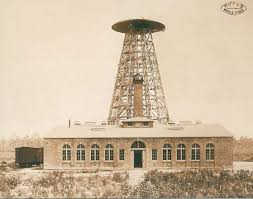
\includegraphics[width=0.41\linewidth]{image6.png}
           
                \caption{Wardenclyffe}
    \label{fig:wardenclyffe}
\end{figure}

 \section{ Nikola Tesla’s Vision (1890s)}
 \quad Nikola Tesla was one of the first pioneers of wireless electricity. In the 1890s, he demonstrated the transmission of electrical energy without wires using resonant inductive coupling. Tesla's famous Tesla Coil was capable of lighting lamps wirelessly from a short distance. He later envisioned the Wardenclyffe Tower to transmit power wirelessly across long distances, although it was never completed.\cite{erickson2020resonant}
 
 \section{Early 20th Century Developments}
 \quad Following Tesla's foundational work, there was minimal practical development in WPT due to technical limitations and the availability of wired alternatives. Some military and aerospace research was carried out mid-century, particularly in radar and RF power transmission for satellites.
 \section{ Microwave Power Transmission (1960s–1980s)}
 \quad NASA and the US Department of Defense explored microwave power transfer (MPT) for long-range applications such as solar-powered aircraft and satellites. In 1964, William C. Brown demonstrated a microwave-powered helicopter, leading to further research into rectenna-based systems and space-based solar power.\cite{zhou2025lowpower}\cite{erickson2020resonant}
 
%%%%%%%%%%%%%%%%%%%%%%%%%%%%%%%%%%%%%%%%%%%%%%%%%%%%%%%%%%%%%%%%%%%%%%%%%%%%%%%%%%%%%%%%%%%%%%%%%%%

% -------------------------

\chapter{Topologies and Working Principle of Wireless Power Transfer}
\vspace{1cm}

\quad Wireless Power Transfer (WPT) enables contactless energy transmission through magnetic or electromagnetic coupling. Its performance depends on the adopted topology and operating principle. This chapter outlines the main WPT topologies and their working mechanisms.

\section{WPT Topologies}

\quad WPT is classified into three primary topologies: Inductive Coupling, Resonant Coupling, and Microwave Power Transfer (MPT).

\subsection{Inductive Coupling}
\begin{figure}[H]
    \centering
    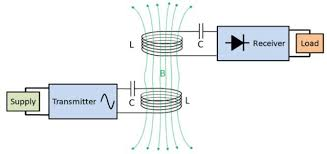
\includegraphics[width=0.6\textwidth]{image1.png}
    \caption{Inductive Coupling Setup}
\end{figure}

\quad Inductive coupling uses magnetic fields between a transmitter and receiver coil. It is efficient at short ranges and common in low-power devices.\cite{erickson2020resonant}

\begin{table}[H]
\centering
\caption{Specifications of Inductive Coupling}
\begin{tabular}{|p{4cm}|p{4cm}|p{6cm}|}
\hline
\textbf{Parameter} & \textbf{Range} & \textbf{Applications} \\
\hline
Transmission Range & 0--10 cm & Smartphones, Toothbrushes \\
\hline
Frequency & 100--500 kHz & Low/moderate power devices \\
\hline
Efficiency & 70--90\% (tight coupling) & Consumer electronics, Medical devices \\
\hline
\end{tabular}
\end{table}

\begin{itemize}
    \item Requires precise coil alignment
    \item Sensitive to lateral misplacement
    \item Used in Qi chargers and wearables
\end{itemize}

\subsection{Resonant Coupling}
\begin{figure}[H]
    \centering
    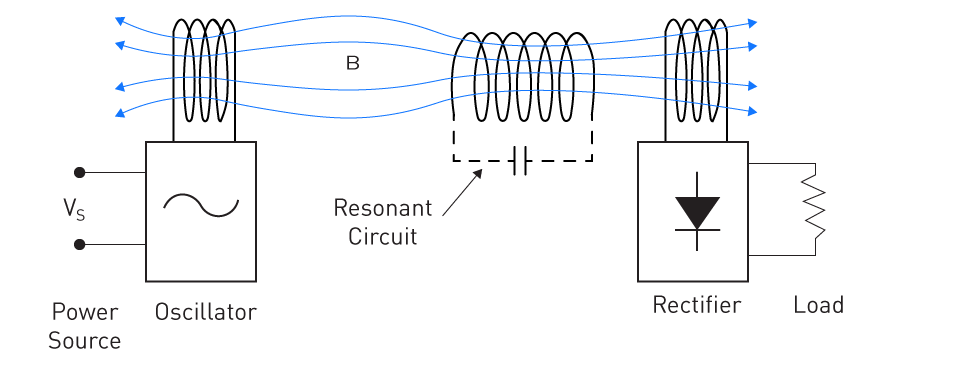
\includegraphics[width=0.6\textwidth]{image.png}
    \caption{Resonant Coupling Setup}
\end{figure}

\quad Resonant coupling improves range and misalignment tolerance by tuning both coils to the same resonant frequency. Topologies include series, parallel, and hybrid networks.\cite{li2022singleended}\cite{erickson2020resonant}

\begin{table}[H]
\centering
\caption{Specifications of Resonant Coupling}
\begin{tabular}{|p{4cm}|p{4.5cm}|p{5.5cm}|}
\hline
\textbf{Parameter} & \textbf{Range} & \textbf{Applications} \\
\hline
Transmission Range & 10--50 cm & EV charging, Wearables \\
\hline
Frequency & 100 kHz--13.56 MHz & Medium/High-power systems \\
\hline
Efficiency & 80--95\% & Robotics, Biomedical implants \\
\hline
\end{tabular}
\end{table}

\begin{itemize}
    \item Provides voltage/current gain via resonant tank
    \item Allows higher spatial tolerance
    \item Widely applied in EV and medical charging
\end{itemize}

\subsection{Microwave Power Transfer (MPT)}
\begin{figure}[H]
    \centering
    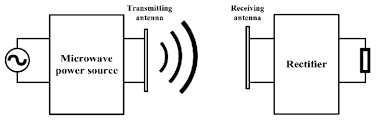
\includegraphics[width=0.6\textwidth]{image3.png}
    \caption{Microwave Power Transfer System}
\end{figure}

MPT employs GHz-frequency waves with rectennas for long-distance transmission.\cite{zhou2025lowpower}

\begin{table}[H]
\centering
\caption{Specifications of MPT}
\begin{tabular}{|p{4cm}|p{5cm}|p{5.2cm}|}
\hline
\textbf{Parameter} & \textbf{Range} & \textbf{Applications} \\
\hline
Transmission Range & Up to km scale & Aerospace, Satellites, Defense \\
\hline
Frequency & 2.4--10 GHz & Long-distance beaming \\
\hline
Efficiency & 30--70\% & Space solar power, UAVs \\
\hline
\end{tabular}
\end{table}

\begin{itemize}
    \item Suitable for long-range transfer
    \item Requires precise beam control
    \item Potential for large-scale space power
\end{itemize}

\section{Working Principle of WPT}

\quad WPT relies on Faraday’s law of electromagnetic induction, enhanced by resonance for higher efficiency.

\subsection{Fundamental Theory}
An alternating current in the transmitter coil induces voltage in the receiver coil:\cite{erickson2020resonant}
\[
V = -N \frac{d\Phi}{dt}
\]
where $N$ is coil turns and $\Phi$ is magnetic flux.

For resonance:
\[
f_r = \frac{1}{2\pi\sqrt{LC}}
\]
\subsection{Power Transfer Mechanism}
Key stages:
\begin{itemize}
    \item Inverter: DC–AC conversion
    \item Transmitter coil: Generates magnetic field
    \item Receiver coil: Captures induced power
    \item Rectifier/regulator: Converts to DC
\end{itemize}

\subsection{Efficiency and Matching}
Efficiency depends on coupling, alignment, and impedance matching:
\[
P = \frac{k^2 \omega^2 L_1 L_2 I_1^2}{R_2 + \left(\omega L_2 - \tfrac{1}{\omega C_2}\right)^2}
\]

\subsection{Factors Affecting Performance\cite{li2022singleended}\cite{bertolini2021frequency}\cite{erickson2020resonant}}
\begin{table}[H]
\centering
\renewcommand{\arraystretch}{1.2}
\begin{tabular}{|p{5cm}|p{10cm}|}
\hline
\textbf{Factor} & \textbf{Impact} \\
\hline
Coupling coefficient $(k)$ & Determines magnetic linkage strength \\
\hline
Coil alignment & Misalignment lowers efficiency \\
\hline
Resonant frequency $(f_r)$ & Optimum frequency maximizes transfer \\
\hline
Quality factor $(Q)$ & Higher $Q$ reduces losses \\
\hline
Impedance matching & Ensures maximum power delivery \\
\hline
Coil spacing & Larger gaps reduce efficiency \\
\hline
Shielding/EMI & Limits interference and leakage \\
\hline
Environment & Metal/dielectric surroundings detune system \\
\hline
\end{tabular}
\caption{Factors Influencing WPT Efficiency}
\end{table}

\chapter{Significance of Resonant Converters in Wireless Energy Transmission}
\vspace{1cm}

\quad Wireless Power Transfer (WPT) requires high efficiency, low EMI, and reliable operation across varying loads and distances. Conventional PWM-based hard-switched converters face high switching losses and degraded high-frequency performance. Resonant converters—primarily Series, Parallel, and Series-Parallel—overcome these limitations and are widely adopted in WPT.

\section{Why Resonant Converters?}

\quad Resonant converters enable soft switching (ZVS/ZCS), reduce EMI, and improve efficiency at high frequencies. Their ability to handle misalignment and varying loads makes them essential in EV and biomedical WPT systems.\cite{irivennela2020wireless}\cite{erickson2020resonant}

\textbf{Key advantages:}
\begin{itemize}
  \item Soft switching with minimal losses
  \item Reduced passive component size
  \item Improved thermal performance
  \item Support for bidirectional power flow (e.g., EV V2G)
  \item Stable operation under variable coil alignment and load
\end{itemize}

\section{Choosing Resonant Topologies for WPT}

\quad Among resonant options, Series, Parallel, and Series-Parallel topologies dominate due to their balance of control simplicity and adaptability.

\begin{table}[H]
\centering
\renewcommand{\arraystretch}{1.2}
\begin{tabular}{|p{4cm}|p{11cm}|}
\hline
\textbf{Topology} & \textbf{Key Features} \\
\hline
Series Resonant & Simple control, efficient under constant loads \\
\hline
Parallel Resonant & Maintains constant current, ideal for variable or biomedical loads \\
\hline
Series-Parallel (Hybrid) & Combines both benefits, highly adaptable for EVs and dynamic coupling \\
\hline
\end{tabular}
\caption{Comparison of Resonant Converter Topologies\cite{lin2021analysis}}
\label{tab:resonant_topologies}
\end{table}

These topologies are preferred over variants such as LCL, LLC, and ZVS-PWM for their robustness, ease of control, and reliable performance across distance and alignment variations. In particular, Series-Parallel converters provide stable power transfer in dynamic wireless environments.\cite{lin2021analysis}\cite{bertolini2021frequency}

% -----------------------------------------------------
\newpage
\section{Advantage of Resonant Converters over Traditional WPT Methods}

\begin{table}[H]
\centering
\renewcommand{\arraystretch}{1.3}
\begin{tabular}{|p{4.5cm}|p{4.5cm}|p{4.5cm}|}
\hline
\textbf{Criteria} & \textbf{Traditional WPT Methods} & \textbf{Resonant Converter-based WPT} \\
\hline
Switching Losses & High due to hard switching & Low due to soft ZVS/ZCS switching \\
\hline
Operating Frequency & Limited to lower frequencies & Efficient at high frequencies \\
\hline
Efficiency & Moderate to low & High, even under partial loading \\
\hline
EMI (Electromagnetic Interference) & High due to sharp switching transitions & Lower due to smoother transitions \\
\hline
Load Adaptability & Poor & Excellent with resonant tuning \\
\hline
Coil Distance Compatibility & Short distances only & Effective over medium air gaps \\
\hline
Control Complexity & Simple & Moderate with AI-based optimization \\
\hline
Component Size & Large passive components & Reduced due to high-frequency operation \\
\hline
Application Suitability & Limited (fixed systems) & Broad (EV, biomedical, robotics, etc.) \\
\hline
\end{tabular}
\caption{Comparison between Traditional and Resonant Converter-based WPT\cite{choi2020resonant}\cite{lin2021analysis}\cite{erickson2020resonant}\cite{irivennela2020wireless}}
\label{tab:comparison_WPT}
\end{table}


% -----------------------------------------------------


%%%%%%%%%%%%%%%%%%%%%%%%%%%%%%%%%%%%%%%%%%%%%%%%%%%%%%%%%%%%%%%%%%%%%%%%%%%%%%%%%%%%%%%%%%%%%%%%%%%

\chapter{Fundamental Working Mechanism of Resonant Converters}
\vspace{1cm}
\section{Working Principle of Resonant Converter}


\quad Resonant converters operate by leveraging the natural oscillatory properties of inductors and capacitors to enable efficient wireless energy transfer. In Wireless Power Transfer (WPT), they ensure energy is transferred across an air gap with minimal loss by maintaining operation at or near the resonant frequency of the circuit. This principle minimizes reactive losses and allows soft switching, enabling high-frequency, high-efficiency performance.\cite{erickson2020resonant}\cite{li2022singleended}

\section{Energy Transfer through Resonance}
\quad At the core of a resonant converter is a tank circuit composed of inductors ($L$) and capacitors ($C$) that oscillate at a specific resonant frequency $f_r$:

\begin{equation}
    f_r = \frac{1}{2\pi\sqrt{LC}}
\end{equation}

This frequency determines the optimal condition for energy exchange between the transmitter and receiver coils. When driven at $f_r$, the system exhibits high voltage and current gain, which is critical in long-distance or low-coupling conditions typical in EV and biomedical applications.\cite{choi2020resonant}

\section{Stage-wise Operation of Resonant Converters}
\quad The operation of resonant converters can be understood in four key stages:\cite{erickson2020resonant}\cite{li2022singleended}\cite{bertolini2021frequency}

\begin{enumerate}
    \item \textbf{DC to AC Conversion:} A high-frequency inverter converts DC power into AC.
    \item \textbf{Resonant Tank Circuit (L-C):} The AC flows through the L-C circuit at resonance for maximum power transfer.
    \item \textbf{Magnetic Coupling:} A transmitting coil creates a magnetic field; a receiving coil tuned to the same frequency captures the energy.
    \item \textbf{AC to DC Conversion:} The received AC is rectified and filtered for DC output.
\end{enumerate}

 
\vspace{0.5cm}

\section{Operating Topologies in Resonant WPT}
\quad The most widely used topologies in WPT systems include Series Resonant Converter (SRC), Parallel Resonant Converter (PRC), and Series-Parallel Resonant Converter (SPRC). These topologies are favored due to their ability to enhance power transfer efficiency, maintain soft-switching conditions, and adapt to varying load and distance conditions. SRCs are ideal for high-power, constant-load applications, PRCs suit biomedical and variable-load systems due to their constant current nature, while SPRCs combine the benefits of both, making them suitable for dynamic environments like electric vehicle charging.







%%%%%%%%%%%%%%%%%%%%%%%%%%%%%%%%%%%%%%%%%%%%%%%%%%%%%%%%%%%%%%%%%%%%%%%%%%%%%%%%%%%%%%%%%%%%%%%%%%%

\chapter{Block Diagram of Resonant Converter-Based Wireless Power Transfer System}
\vspace{0.5cm}
\begin{center}

\end{center}
\quad Wireless Power Transfer (WPT) systems based on resonant converters follow a multi-stage energy conversion process to ensure efficient power delivery across an air gap. The architecture is modular, enabling the use of high-frequency switching and magnetic resonance for enhanced performance.

\begin{figure}[H]
    \centering
    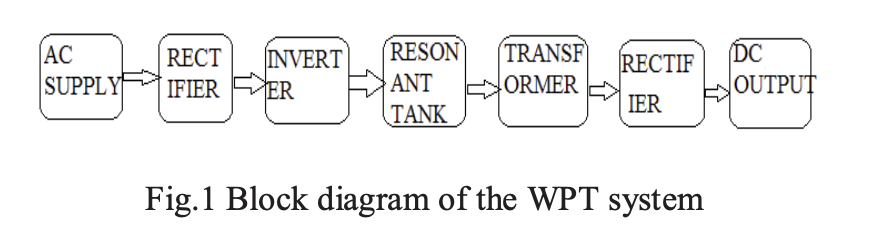
\includegraphics[width=0.9\textwidth]{Untitled.png} % Replace with your figure filename
    \caption{Block diagram of the resonant converter-based WPT system\cite{irivennela2020wireless}}
    \label{fig:wpt_block}
\end{figure}

\section{Functional Description of Each Stage}
\quad Wireless Power Transfer (WPT) systems based on resonant converters follow a multi-stage energy conversion process to ensure efficient power delivery across an air gap. The modular architecture facilitates high-frequency switching and magnetic resonance, optimizing performance in terms of energy efficiency, electromagnetic compatibility, and system adaptability.\cite{irivennela2020wireless}


\begin{table}[H]
\centering
\renewcommand{\arraystretch}{1.3}
\begin{tabular}{|p{4.5cm}|p{10.5cm}|}
\hline
\textbf{Block} & \textbf{Functionality Description} \\
\hline
\textbf{AC Supply} & The system begins with a standard AC input, typically from the grid (50/60 Hz). \\
\hline
\textbf{Rectifier (Input)} & Converts the low-frequency AC to DC using diode or controlled rectifiers. This DC voltage serves as the input to the inverter. \\
\hline
\textbf{High-Frequency Inverter} & Converts the DC signal into high-frequency AC, enabling resonance in the following stage. Soft-switching topologies (ZVS/ZCS) improve efficiency. \\
\hline
\textbf{Resonant Tank Circuit} & An LC network designed to resonate at a specific frequency (typically 6.78 MHz), allowing efficient energy transfer with minimum losses. \\
\hline
\textbf{High-Frequency Transformer} & Provides galvanic isolation and steps up/down the AC voltage. Operates at resonant frequency, minimizing core losses. \\
\hline
\textbf{Rectifier (Output)} & Converts the received AC back into DC using high-frequency rectifiers. This stage often uses synchronous rectification for better efficiency. \\
\hline
\textbf{DC Output to Load} & The final regulated DC output is fed to the load (e.g., EV battery or device). May include voltage regulation or battery management systems. \\
\hline
\end{tabular}
\caption{Functional Blocks and Description of a Resonant WPT System}
\label{tab:WPT_block_functionality}
\end{table}

%%%%%%%%%%%%%%%%%%%%%%%%%%%%%%%%%%%%%%%%%%%%%%%%%%%%%%%%%%%%%%%%%%%%%%%%%%%%%%%%%%%%%%%%%%%%%%%%%%%

\chapter{Types of Resonant Converters for Wireless Power Transfer}
\vspace{1cm}
\quad Resonant converters are essential in wireless power transfer (WPT) systems due to their high efficiency, compact size, and capability to operate at high frequencies. These converters utilize the resonance of inductive and capacitive elements to transfer power efficiently across the air gap. Depending on the configuration and requirements of the application, resonant converters can be categorized into several topologies. These are mainly classified into Series Resonant, Parallel Resonant, and Series-Parallel Resonant topologies. This classification is based on extensive studies and comparative analyses found in IEEE reference materials and technical slides related to EV wireless charging.

\section{Series Resonant Converter (SRC)}

\quad The Series Resonant Converter features inductors and capacitors connected in series with the load. It operates efficiently at resonant frequency and provides high voltage gain. SRC is widely used where the load remains relatively constant, as observed in early-generation EV charging prototypes.\cite{li2022singleended}\cite{erickson2020resonant}

\begin{itemize}
    \item Suitable for high-voltage applications.
    \item Offers Zero Voltage Switching (ZVS) and Zero Current Switching (ZCS).
    \item Simple control but poor regulation under variable loads.
    \item Reduced EMI due to soft switching.
\end{itemize}

\section{Parallel Resonant Converter (PRC)}

\quad In the Parallel Resonant Converter, the capacitor is connected in parallel to the load. It provides a constant current output characteristic, making it suitable for applications where load varies significantly, such as biomedical implants and mobile charging pads.\cite{choi2020resonant}\cite{bertolini2021frequency}

\begin{itemize}
    \item Better load regulation.
    \item Higher circulating current compared to SRC.
    \item Suitable for constant current applications.
    \item Requires careful design to avoid component overrating.
\end{itemize}

\section{Series-Parallel Resonant Converter (SPRC)}

\quad The Series-Parallel Resonant Converter combines the benefits of both SRC and PRC by connecting part of the resonant capacitor in series and part in parallel. This hybrid structure offers a compromise between constant current and constant voltage operation.\cite{lin2021analysis}\cite{li2022singleended}

\begin{itemize}
    \item Good performance over a wide range of load conditions.
    \item Enhanced efficiency and better control.
    \item Commonly used in Electric Vehicle (EV) wireless charging.
    \item Supports dynamic alignment in inductive coupling systems.
\end{itemize}


%%%%%%%%%%%%%%%%%%%%%%%%%%%%%%%%%%%%%%%%%%%%%%%%%%%%%%%%%%%%%%%%%%%%%%%%%%%%%%%%%%%%%%%%%%%%%%%%%

\chapter{Series Resonant Converter for Wireless Power Transfer}
\vspace{1cm}
\section{Introduction}
\quad The Series Resonant Converter (SRC) employs a series LC tank circuit driven by a high-frequency inverter, making it well-suited for efficient Wireless Power Transfer (WPT). Its resonant operation enables soft switching (ZVS/ZCS), reducing switching losses and EMI.\cite{li2022singleended}\cite{erickson2020resonant}

\begin{figure}[H]
    \centering
    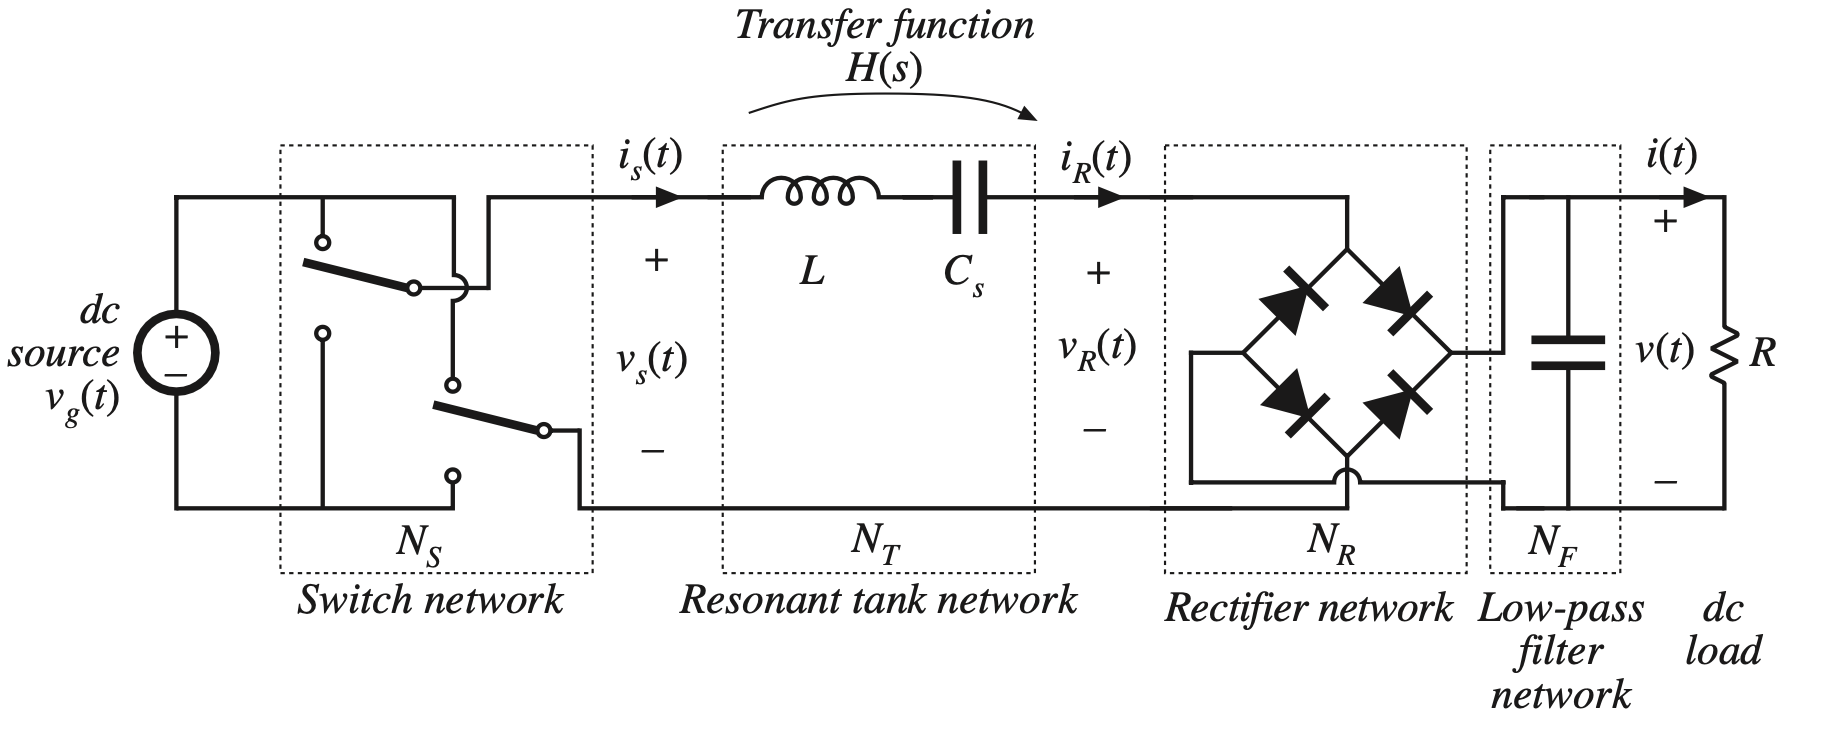
\includegraphics[width=0.7\linewidth]{788.png}
    \caption{Series Resonant Converter (SRC) Topology}
\end{figure}

 In SRCs, a half-bridge or full-bridge inverter excites the LC tank with high-frequency AC. The rectifier and filter at the output deliver regulated DC to the load. Operation near resonance ensures high efficiency and compact passive design.

\section{Working Principle}
The resonant tank is governed by:
\[
f_r = \frac{1}{2\pi \sqrt{L_r C_r}}
\]

\begin{itemize}
    \item At \(f_s = f_r\): Tank impedance is minimum and resistive; current and voltage are in phase, maximizing transfer.
    \item For \(f_s < f_r\): Capacitive mode, enabling ZVS.
    \item For \(f_s > f_r\): Inductive mode, enabling ZCS.
\end{itemize}

Thus, by controlling the switching frequency \(f_s\), the SRC regulates power flow and supports soft switching across operating conditions.\cite{li2022singleended}

\section{Advantages and Limitations}

\subsection*{Advantages}
\begin{itemize}
    \item Intrinsic ZVS/ZCS for reduced switching loss.
    \item Low EMI due to sinusoidal current waveforms.
    \item High efficiency and thermal reliability at HF operation.
    \item Compact design with smaller passive elements.
    \item Tolerant to coil misalignment in WPT systems.\cite{irivennela2020wireless}\cite{li2022singleended}\cite{lin2021analysis}\cite{erickson2020resonant}
    
\end{itemize}

\subsection*{Limitations}
\begin{itemize}
    \item Output voltage sensitive to load variations.
    \item Efficiency drops under light-load conditions.
    \item Requires precise \(L_r\)–\(C_r\) tuning and complex control.
    \item Higher device voltage stress than parallel topologies.\cite{irivennela2020wireless}\cite{li2022singleended}\cite{lin2021analysis}\cite{erickson2020resonant}
\end{itemize}

\section{Design }
Key parameters include resonant frequency and characteristic impedance:
\[
f_r = \frac{1}{2\pi \sqrt{L_r C_r}}, \quad Z_r = \sqrt{\tfrac{L_r}{C_r}}
\]

Design trade-offs:
\begin{itemize}
    \item \(f_s < f_r\): Capacitive mode (ZVS, high efficiency at heavy load).
    \item \(f_s > f_r\): Inductive mode (ZCS, useful for light load/charging).
    \item \(f_s = f_r\): Maximum power transfer with unity PF.
    \cite{bertolini2021frequency}
\end{itemize}

\section{Applications in WPT}
SRCs are preferred where high frequency, compactness, and efficiency are critical:
\begin{itemize}
    \item \textbf{Medical implants}: Efficient power delivery with minimal tissue heating.
    \item \textbf{Consumer electronics}: Portable device charging via resonant coils.
    \item \textbf{EV wireless charging (low to mid-power)}: Robust transfer across moderate misalignments.
    \cite{choi2020resonant}
\end{itemize}

%%%%%%%%%%%%%%%%%%%%%%%%%%%%%%%%%%%%%%%%%%%%%%%%%%%%%%%%%%%%%%%%%%%%%%%%%%%%%%%%%%%%%%%%%%%%%%%%%%%

\chapter{Parallel Resonant Converter for Wireless Power Transfer}
\vspace{1cm}
\section{Introduction}
\quad The Parallel Resonant Converter (PRC) is a resonant power converter topology used in wireless power transfer systems where the resonant capacitor is placed in parallel with the load. This arrangement supports near-constant current characteristics, making it suitable for applications like biomedical implants, LED drivers, and low-power charging.In PRC, an inductor (\(L_r\)) and a capacitor (\(C_r\)) form a parallel resonant tank connected across the load. The converter is typically driven by a high-frequency inverter, which enables resonance in the LC tank circuit, promoting efficient energy transfer with reduced switching losses.\cite{erickson2020resonant}\cite{li2022singleended}


\begin{figure}
        \centering
        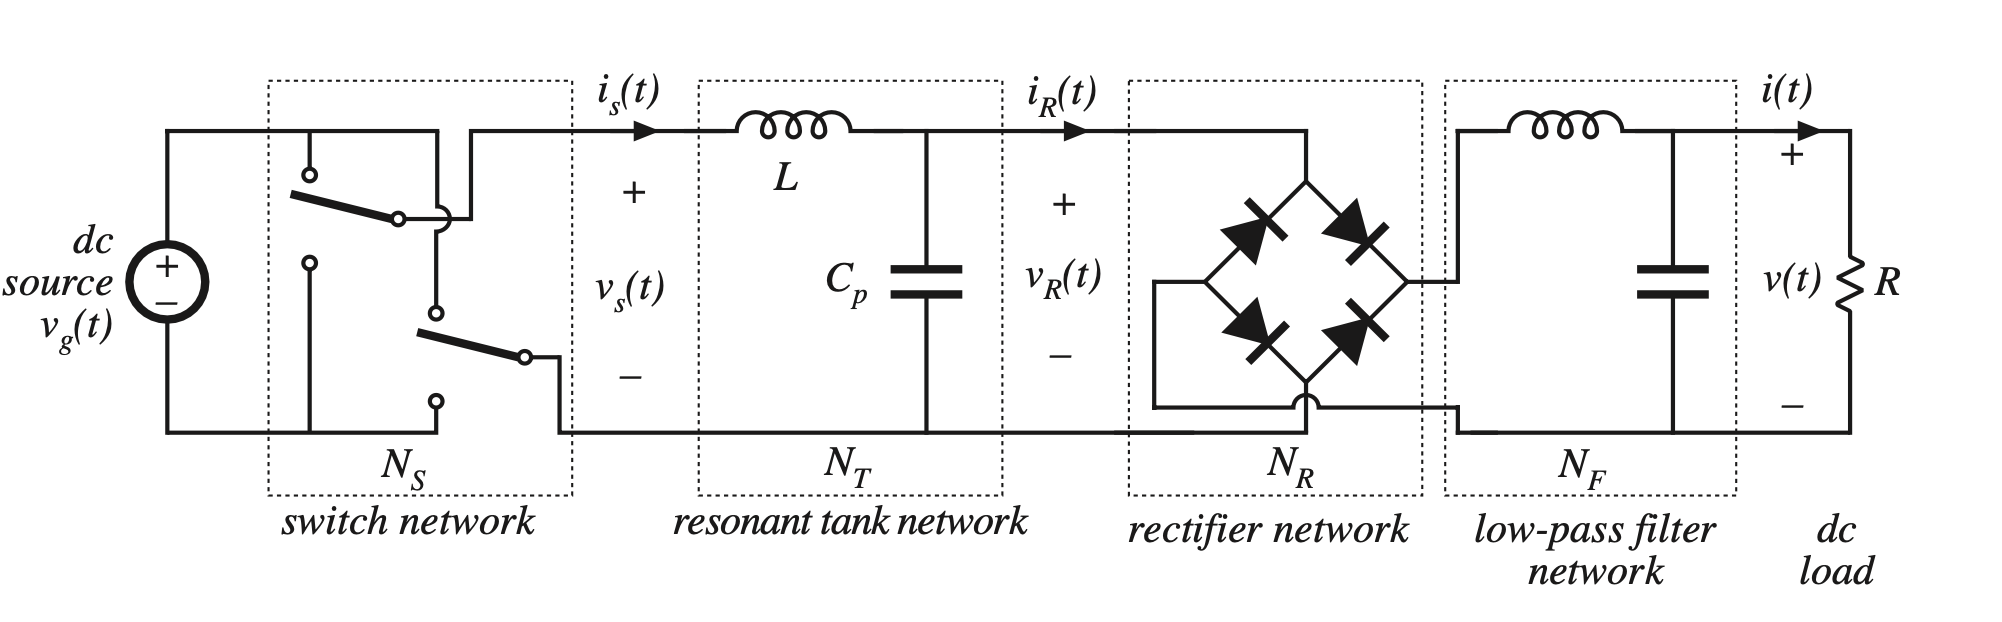
\includegraphics[width=0.65\linewidth]{6677.png}
      
        \caption{Circuit Diagram of a Parallel Resonant Converter}
\end{figure}

\section{Working }

\quad The PRC operates by exciting the LC tank at or near its natural resonant frequency:

\[
f_r = \frac{1}{2\pi \sqrt{L_r C_r}}
\]

At resonance, the impedance of the tank circuit is minimum, allowing efficient power transfer to the load. Since the capacitor is in parallel with the load, the voltage across the capacitor is the same as the output voltage, while the inductor determines the current flow.\cite{irivennela2020wireless}

\begin{itemize}
    \item At \(f = f_r\), the tank circuit draws maximum current.
    \item Operating slightly above resonance (\(f > f_r\)) enables Zero Current Switching (ZCS).
    \item Load voltage is regulated via frequency control.
\end{itemize}



\section{Advantages and Disadvantages}

\subsection*{Advantages}

\begin{itemize}
    \item Delivers nearly constant output current — ideal for LEDs and implants.
    \item Supports ZCS, minimizing switching losses and EMI.
    \item Inherent current-limiting protects sensitive loads.
    \item Soft-switching and low-noise compatible.
    \item Easy control via frequency tuning.\cite{choi2020resonant}\cite{li2022singleended}\cite{lin2021analysis}
\end{itemize}

\subsection*{Disadvantages}
\begin{itemize}
    \item Higher circulating current increases conduction losses.
    \item Needs larger passive components.
    \item Less efficient in high-power scenarios.
    \item Voltage regulation is load-sensitive.
    \item Poor handling of wide load variations without advanced control.\cite{choi2020resonant}\cite{li2022singleended}\cite{lin2021analysis}
\end{itemize}

\section{Design }

\quad The resonant frequency is determined by the LC values as:

\[
f_r = \frac{1}{2\pi \sqrt{L_r C_r}}
\]

\quad The equivalent impedance seen by the inverter is:

\[
Z_{eq} = \left( \frac{1}{j\omega C_r} + R_{load} \right)
\]

\quad The operating frequency is selected to balance:
\begin{itemize}
    \item Soft-switching conditions (ZCS preferred),
    \item Minimum circulating current,
    \item Load voltage regulation.\cite{choi2020resonant}
\end{itemize}

\section{Applications in Wireless Power Transfer}



Common applications include:

\begin{itemize}
    \item \textbf{Biomedical Implants}: Safe and reliable low-power energy delivery.
    \item \textbf{LED Lighting Systems}: Stable current source for consistent brightness.
    \item \textbf{Precision Charging}: Low-power IoT or wearable device charging.\cite{choi2020resonant}
\end{itemize}




%%%%%%%%%%%%%%%%%%%%%%%%%%%%%%%%%%%%%%%%%%%%%%%%%%%%%%%%%%%%%%%%%%%%%%%%%%%%%%%%%%%%%%%%%%%%%%%%%%%

 

\chapter{Series-Parallel Resonant Converter for Wireless Power Transfer}
\vspace{1cm}\section{Introduction}

\quad The Series-Parallel Resonant Converter (SPRC), also known as the hybrid resonant converter, combines the characteristics of both series and parallel resonant circuits. It is widely used in medium to high-power wireless power transfer (WPT) applications where both constant current and constant voltage characteristics may be required depending on the load conditions.In SPRC topology, the resonant tank consists of a combination of series and parallel LC components. Typically, a capacitor is placed in parallel with the load, while another capacitor and inductor are placed in series with the input. This topology aims to balance the high efficiency of series converters with the current regulation of parallel converters.\cite{irivennela2020wireless}\cite{li2022singleended}


\begin{figure}
        \centering
        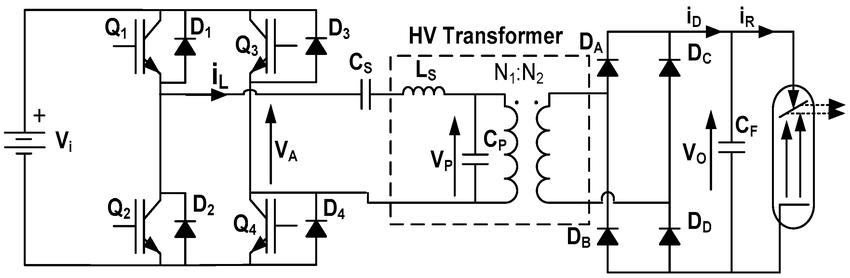
\includegraphics[width=0.65\linewidth]{image00.png}
       
        \caption{Circuit Diagram of a Series-Parallel Resonant Converter}
\end{figure}

\section{Working Principle}

\quad The SPRC is excited by a high-frequency AC voltage from an inverter. The resonant tank is tuned to a resonant frequency determined by both the series and parallel branches. The presence of both types of capacitive coupling allows the system to adapt more flexibly to load variations.\cite{choi2020resonant}

\[
f_r = \frac{1}{2\pi \sqrt{L_r C_{eq}}}
\]

\quad Where \(C_{eq}\) depends on the interaction of series and parallel capacitors.

\quad Key features of operation:

\begin{itemize}
    \item At light loads, the circuit behaves more like a parallel resonant converter, providing constant current output.
    \item At heavy loads, it tends to behave like a series resonant converter, favoring efficiency.
    \item Load regulation is achieved by shifting the operating frequency above or below the resonant point.
\end{itemize}


\section{Advantages and Disadvantages}

\subsection*{Advantages}
\begin{itemize}
    \item Balances constant voltage and current output.
    \item Adapts well to variable loads.
    \item Supports ZVS/ZCS over a broad range.
    \item Robust under dynamic charging conditions.\cite{bertolini2021frequency}\cite{lin2021analysis}\cite{erickson2020resonant}
\end{itemize}

\subsection*{Disadvantages}
\begin{itemize}
    \item Complex due to dual-mode resonance.
    \item Difficult tuning for varying loads.
    \item More passive components raise cost and size.
    \item Needs advanced control strategies.\cite{bertolini2021frequency}\cite{lin2021analysis}\cite{erickson2020resonant}
\end{itemize}

\section{Design Parameters}

\quad Design of SPRC involves calculating the resonant frequencies for both branches:

\[
f_s = \frac{1}{2\pi \sqrt{L_r C_s}}, \quad f_p = \frac{1}{2\pi \sqrt{L_r C_p}}
\]

Where:

- \(L_r\) is the shared resonant inductor,
- \(C_s\) is the series capacitor,
- \(C_p\) is the parallel capacitor.

\quad The converter typically operates at a frequency between \(f_s\) and \(f_p\) to optimize power transfer and regulation.

\section{Applications in Wireless Power Transfer}



Use cases of SPRC in WPT include:

\begin{itemize}
    \item \textbf{Electric Vehicle (EV) Charging}: Dynamic range and high efficiency.
    \item \textbf{Consumer Electronics}: Adaptive power delivery to variable loads.
    \item \textbf{Industrial Automation}: Reliable charging in noisy or variable environments.\cite{irivennela2020wireless}
\end{itemize}


 

\chapter{Efficiency Factors in Resonant Converter Based WPT}
\vspace{1cm}

The efficiency of resonant Wireless Power Transfer (WPT) systems is influenced by several interdependent electrical and physical parameters. Optimizing these factors is essential for maximizing power transfer and minimizing losses.

\section{Operating Frequency and Resonant Tuning}  
Maximum efficiency is achieved when the system operates at its tank resonance, defined by 
\[
\omega_0 = \frac{1}{\sqrt{LC}}.
\] 
Any deviation from this resonant frequency increases reactive power losses, thereby reducing transfer efficiency. Maintaining precise resonance is critical for optimal performance.\cite{irivennela2020wireless}

\section{Quality Factor (\(Q\))}  
The quality factor, given by 
\[
Q = \frac{\omega_0 L}{R},
\] 
directly affects efficiency. Higher \(Q\) values result in sharper resonance and higher efficiency. However, excessively high \(Q\) narrows the bandwidth, which can degrade load regulation and make the system sensitive to variations.\cite{choi2020resonant}

\section{Coupling Coefficient (\(k\)) and Mutual Inductance (\(M\))}  
The coupling coefficient 
\[
k = \frac{M}{\sqrt{L_1 L_2}}
\] 
determines the strength of magnetic coupling between transmitter and receiver coils. Strong coupling improves power transfer but reduces misalignment tolerance. Weak coupling reduces efficiency, especially for larger coil separations.

\section{Load Impedance Matching}  
Maximum power transfer occurs when the load impedance \(Z_L\) matches the source impedance \(Z_s\). Impedance mismatch causes reflections and power loss. Adaptive tuning networks or frequency control can compensate for variable loads.\cite{erickson2020resonant}\cite{bertolini2021frequency}

\section{Switching Losses and Soft Switching}  
High-frequency operation increases switching stress in power electronic devices. Techniques such as Zero-Voltage Switching (ZVS) and Zero-Current Switching (ZCS) minimize transition losses and suppress electromagnetic interference (EMI), thereby improving efficiency.\cite{irivennela2020wireless}

\section{Conduction Losses in Passive Components}  
Conduction losses in passive elements are expressed as 
\[
P_{loss} = I^2 R.
\] 
Parasitic resistance of inductors and capacitors contributes to these losses. Using low-ESR capacitors and high-\(Q\) inductors reduces conduction losses and improves overall efficiency.

\section{Coil Geometry and Design}  
Coil parameters—including turns, spacing, and geometry—affect coupling and resistance. Litz wire mitigates skin and proximity effects at high frequencies, while proper shielding reduces eddy currents and stray fields.

\section{Modulation and Control Strategy}  
Efficiency is also influenced by the modulation and control strategy. Techniques such as Frequency Modulation (FM), Phase-Shift Modulation (PSM), and Pulse-Density Modulation (PDM) optimize performance. Adaptive real-time tuning helps maintain high efficiency under load and alignment variations.\cite{erickson2020resonant}

\section{Typical Efficiency Levels}  
Resonant converters in WPT typically achieve high efficiencies. Series Resonant Converters (SRC) operate around 85–95\%, Parallel Resonant Converters (PRC) around 80–90\%, and Series-Parallel Resonant Converters (SPRC) achieve 88–95\%.

\begin{table}[H]
    \centering
    \caption{Efficiency Ranges of Resonant Converters in WPT}
    \begin{tabular}{|c|c|}
        \hline
        \textbf{Converter Type} & \textbf{Efficiency (\%)} \\
        \hline
        Series Resonant (SRC) & 85–95 \\
        Parallel Resonant (PRC) & 80–90 \\
        Series-Parallel Resonant (SPRC) & 88–95 \\
        \hline
    \end{tabular}
\end{table}

\chapter{Applications, Challenges, and Future Trends}
\vspace{1cm}

\section{Applications}

Resonant converter-based WPT systems are widely used due to their efficient high-frequency operation and soft-switching capability. Applications span transportation, consumer electronics, healthcare, industrial automation, and aerospace.

\subsection{Electric Vehicle (EV) Charging}
Resonant converters form the backbone of modern EV wireless charging, supporting both static and dynamic modes:
\begin{itemize}
    \item \textbf{Static Charging:} Used in stationary EV chargers to maximize transfer efficiency and minimize switching stress.  
    \item \textbf{Dynamic Charging:} Series resonant converters provide stable operation for moving vehicles, accommodating variable loads and alignment.  \cite{irivennela2020wireless}
\end{itemize}

\subsection{Consumer Electronics}
Parallel resonant converters are commonly integrated into wireless charging pads for smartphones, wearables, and tablets, ensuring electrical isolation, user safety, and stable voltage regulation under varying loads.\cite{li2022singleended}

\subsection{Biomedical Implants}
Series-parallel resonant converters enable reliable power delivery to medical implants such as pacemakers and neurostimulators, providing consistent current/voltage despite body-induced coil misalignment.

\subsection{Industrial Robotics and Automation}
Resonant WPT powers moving and rotating robotic arms, eliminating mechanical connectors, reducing wear, preventing sparking, and enhancing safety in automated environments.

\subsection{Aerospace and Defense}
High-frequency resonant WPT enables wireless powering of UAVs, satellites, and remote sensor nodes, facilitating long-range, maintenance-free energy transfer where wired solutions are impractical.\cite{bertolini2021frequency}

\section{Challenges}

Despite their advantages, resonant WPT systems face several technical and practical challenges:  
\begin{itemize}
    \item \textbf{Load and Distance Sensitivity:} Series resonant converters are highly dependent on load variations and coil spacing.  
    \item \textbf{Misalignment Losses:} Lateral or angular coil misalignment reduces mutual inductance and efficiency.  
    \item \textbf{Complex Feedback Control:} Continuous frequency or impedance tuning is needed to maintain resonance in dynamic conditions.  
    \item \textbf{Thermal Management:} High conduction and switching losses require advanced cooling solutions.  
    \item \textbf{Electromagnetic Interference (EMI):} MHz-range operation introduces EMI concerns, necessitating shielding and filtering.  
    \item \textbf{Light-Load Inefficiency:} Parallel resonant converters often suffer reduced efficiency under low or no-load conditions.  
\end{itemize}

\section{Future Trends}

The future of resonant WPT emphasizes enhanced adaptability, smarter control, and wider industrial deployment. Research focuses on miniaturization, dynamic charging, and advanced materials:  
\begin{itemize}
    \item \textbf{AI-Based Tuning:} Machine learning for adaptive resonance tracking and predictive load management.  
    \item \textbf{Multi-Device Systems:} Frequency or time-division multiplexing to power multiple receivers simultaneously.   
    \item \textbf{Dynamic EV Charging:} Embedded roadway coils enabling real-time vehicle powering.  
    \item \textbf{Hybrid Topologies:} Combining series and parallel designs to improve adaptability and load regulation.  
    \item \textbf{Material Innovations:} Use of metamaterials and advanced ferrites for high-efficiency, compact coils.  
    \item \textbf{Standardization:} Development of global interoperability and safety standards for WPT deployment.  
\end{itemize}

\chapter{Conclusion}

\section{Conclusion}
\vspace{1cm}
\quad Resonant converter-based Wireless Power Transfer (WPT) has emerged as a highly efficient, contactless method for delivering power across various sectors such as electric mobility, biomedical devices, and consumer electronics. Utilizing magnetic resonance and soft-switching techniques, these systems minimize switching losses and improve power density, especially at high frequencies.

\quad Different resonant topologies offer specific advantages: Series converters handle variable loads well, Parallel topologies provide better voltage control and safety, while Series-Parallel types offer a balance of efficiency and regulation. However, key challenges remain, including sensitivity to coil alignment, variations in coupling, electromagnetic interference (EMI), and the need for precise control and thermal management.

\quad Ongoing research is addressing these limitations through innovations such as AI-integrated adaptive tuning, advanced coil geometries using metamaterials, and dynamic charging platforms for in-motion EVs. Efforts toward standardization, safety compliance, and system interoperability are also crucial for real-world deployment.

\quad In summary, resonant Converter based WPT is a transformative approach with significant potential to redefine modern power systems. As technology evolves and interdisciplinary collaboration grows, these systems are expected to become a cornerstone of next-generation, sustainable, and flexible energy infrastructures.

%%%%%%%%%%%%%%%%%%%%%%%%%%%%%%%%%%%%%%%%%%%%%%%%%%%%%%%%%%%%%%%%%%%%%%%%%%%%%%%%%%%%%%%%%%%%%%%%%%%
\newpage


% Patch the bibliography command to add space

% Patch bibliography to add vertical space above and below title

% Adjust bibliography title and spacing
\makeatletter
\patchcmd{\thebibliography}{\chapter*{\bibname}}{\chapter*{\bibname}\vspace{2em}}{}{}
\makeatother
\renewcommand{\bibname}{Reference} % Title



\nocite{*}
\bibliographystyle{ieeetr}
\bibliography{bib}

\newpage
\begin{center}

   {\Large \textit{Vision and Mission of the Institute}} \\[1em]

\end{center}



\noindent\textbf{Vision:} Be a centre of Technological Excellence for the betterment of society.

\vspace{1em}

\noindent\textbf{Mission:} To impart professional education to students from all sectors of the society to
mould them to be competent, committed, research-oriented, and socially responsible citizens capable of deploying technology for the goodwill of society.

 

\begin{center}

   {\Large \textit{Vision and Mission of the Department of Electrical \\ and Electronics Engineering}} \\[1em]

\end{center}

 

\noindent\textbf{Vision:} To be a centre of technological excellence in Electrical and Electronics Engineering for the betterment of society.\\[0.5em]

 

\noindent\textbf{Mission:}

\begin{itemize}

 \item \textbf{M1:} To bestow high-quality education through excellence in its faculty and facilities.

 \item \textbf{M2:} To transform young minds into competent and full-fledged professionals.

 \item \textbf{M3:} To nurture ethical values.

 \item \textbf{M4:} To invoke a passion to serve the society.

\end{itemize}

 

 

 

\end{document}